% Author: Matthew Turner

% \documentclass[11pt,letterpaper]{article}
\documentclass[letterpaper,11.5pt]{scrartcl}
% \documentclass[11pt]{report}
% \documentclass{report}
% \documentclass{book}
\usepackage[bookmarks, hidelinks]{hyperref}
\usepackage{amssymb,amsmath}
% \usepackage{fullpage}
\usepackage{tabulary}
\usepackage{tabularx}
\usepackage{float}
% \usepackage[margin=1.00in]{geometry}
\usepackage[margin=0.90in]{geometry}

\usepackage{caption}
\usepackage{booktabs}
\usepackage{pslatex}
\usepackage{apacite}
\usepackage{subcaption}
\usepackage{pgfplots}
\usepackage{wrapfig}
\usepackage[english]{babel}
\usepackage{lmodern}
\usepackage{setspace}
\doublespace
% \usepackage{url}
\usepackage{bigfoot}
\usepackage[export]{adjustbox}
\setlength\intextsep{0pt}

\usepackage{graphicx}

\title{Some forms of uncertainty may suppress the evolution of social learning}

\author{{}}

\begin{document}
\maketitle


\begin{abstract}

Social learning is essential to survival. It is likely to evolve when it is more
efficient than asocial, trial-and-error learning. The consensus in cultural
evolutionary theory holds that some amount of environmental variability and
uncertainty about the best decisions are necessary for social learning to evolve.
However, current models for the evolution of social learning tend to conflate forms
of uncertainty, and rarely consider different ones in tandem. Moreover, many models
are limited by considering only two possible behaviors and environmental states.
Here we use evolutionary agent-based modeling to improve on these shortcomings. We
model a time-varying environment with dozens of possible behaviors performed by
agents engaging in individual and social learning. We show that ambiguous payoffs,
larger possible decision sets, and shorter agent lifespans sometimes increase social
learning prevalence, as expected. However, we also find that, under some conditions,
these forms of uncertainty can select against social learning.
\end{abstract}

\section{Introduction}

Social learning is essential to human and other species' everyday life and survival.
It allows individuals to solve problems when acquiring information from others is more efficient than learning
on one's own~\cite{Laland2004}. Theory predicts that social
learning should be favored in contexts with greater
uncertainty~\cite{BoydRicherson1985,Henrich1998}, and this prediction has received some empirical support~\cite{McElreath2005,Kendal2018}. 
However, the meaning of the term ``uncertainty'' is not always clear, and often conflates environmental variability, spatial heterogeneity, and ambiguity or uncertainty about payoff structure. 
Moreover, most models of the evolution of social learning ``blackbox'' key 
cognitive learning processes that underlie it~\cite{Heyes2016}. 

In this paper we use agent-based modeling to compare the effect of
different sources of uncertainty on social learning
by ``unblackboxing'' typically abstracted-out model components 
of environmental variability, payoff structures and
agent life histories, and  learning mechanisms. ``Uncertainty''  
means variability where the probabilistic structure is unknown. %cannot be learned.
Uncertainty increases when payoffs are more similar across behaviors, when
environmental variability increases, when the number of possible behaviors
increases, and when lifespan decreases.  In this paper we show that more ambiguous
payoff structures and shorter lifespans sometimes do lead to greater reliance on
social learning---however, we also identify and explain cases where greater
uncertainty leads to less social learning due to the possibility that social
information is misleading.  We thus conclude that many predictions made by previous
models of the evolution of social learning are likely overgeneralized.
%~\cite{Yarkoni2021}. 

\subsection{Social Learning}

Social learning, as we consider it here, occurs whenever an individual acquires a behavior by observing another individual. This need not require explicit instruction, and is, in fact, widespread across a broad range of nonhuman 
taxa~\cite{Kendal2018,Allen2019}. Importantly, social information can be inherited both
from parents --- i.e., via \emph{vertical transmission} like genetic information --- and
from others in the same generation --- i.e., via \emph{horizontal transmission}
\cite{CavalliFeldman1981}. The joint action of vertical and horizontal transmission
gives rise to qualitatively different evolutionary dynamics. For example,
inter-generational environmental change will affect the adaptive value of genetic
information and vertically-transmitted cultural information more than information
that is horizontally transmitted. We include both horizontal and vertical transmission pathways in our
model. For simplicity, we ignore oblique transmission in which non-parental members
of the previous generation are observed.

Environmental variability has been seen as a key selective force in shaping social learning starting with the first formal models of cultural evolution~\cite{CavalliFeldman1981,BoydRicherson1985}.
Totally stable environments will not favor learning mechanisms because information can become genetically hardwired, while  extreme environmental instability will degrade the value
of social learning as information becomes rapidly outdated~\cite{Feldman1996}. This suggests that an intermediate degree of environmental predictability will favor social learning. Strategies can also evolve to mitigate the risks of relying on outdated social information by weighing more heavily information from others who more recently acquired it~\cite{Rendell2010}.

Uncertainty has also been modelled as arising from other aspects of the environment. 
For example, \citeA{Perreault2012} vary the ambiguity of the environmental cue individuals get through individual learning about the state of the world. Perhaps not surprisingly, the more ambiguous the asocial information, the greater the selection for weighing social information heavily. Alternatively, uncertainty about the optimal behavior has been modelled by increasing the number of cultural traits to choose from. 

Empirical research supports some of these theoretical predictions. Organisms flexibly use social learning as a function of the ambiguity of the environmental cue and of other environmental features that are often subsumed under the rubric of ``uncertainty.''
While some studies explicitly impose a cost whenever participants use asocial
information \cite{Morgan2012,atkisson_etal2012}, 
others allow the costs of each strategy to emerge as a function of task structure and assess its consequences for learning strategies. 
For example, when participants received equivocal private information about the best investment to make in a lab game,
they were more likely to rely on social information to make their choice~\cite{Toelch2013}. 
\citeA{McElreath2005} developed a similar experiment where participants ``pulled'' virtual slot machine arms (often called ``bandits''), each yielding stochastic payoffs. Participants relied more on social learning when the bandits had higher-variance payoffs, and when the highest-paying bandit changed more frequently. 
The number of options to choose between can also increase uncertainty about the optimal choice, and has been shown to increase participants' reliance on social learning \cite{Muthukrishna2016a}. 

Thus existing theoretical work and the empirical evidence seem to support that various forms of uncertainty favor the evolution of social learning. However, uncertain outcomes are operationalized in different ways across models, and any given model tends to focus on only one or two forms of uncertainty at a time. Our agent-based modeling approach enables us to explicitly specify different forms of uncertainty independently in order to understand which of these environmental factors particularly favor the evolution of social learning. Simultaneous modelling also allows us to examine their interaction. We first attempt conceptual replications of previous models' findings, and then examine where they diverge.

\subsection{Research overview}

Computational agents in our model face a problem: every time step they perform
one of several behaviors, with each behavior represented by a ``bandit'' that
pays off 1 or 0 with some probability. One of these behaviors (the optimal
behavior) pays off with a higher probability than all the others.
Agents decide which behavior to 
perform based either on a success-biased observation 
of a peer's behavior (social learning) or based on their own observations (asocial learning).
Agents then update their memory of expected payoffs for each behavior 
when they receive a payoff from their chosen
action. Within this framework we have four mechanisms by which we operationalize 
and vary uncertainty:
(1) the expected payoffs of the optimal behavior and all the rest---when payoffs
are nearly identical, uncertainty in the form of ambiguity increases; (2) the
environmental variability, i.e., the probability that the optimal behavior 
changes between generations; (3) the number of possible behaviors the environment allows---which
behavior is optimal is more uncertain when there are more possibilities; and (4)
 agent lifespan---agents experience fewer learning opportunities and die more uncertain about which behavior
is optimal when their lifespan is shorter. 

The primary outcome measure of our
model is the average difference between the frequency of (horizontal) 
social learning and the frequency of asocial
learning across all agents. If social learning is more prevalent than asocial
learning this suggests that the optimal behavior is more likely found
by copying peers than by trial-and-error search.
Conversely, when asocial learning is more prevalent, this suggests social information
is likely to be misleading. 
When social and asocial learning are 
equally prevalent this means there is no discernible advantage to either, i.e.,
the agents have weak priors on which channel provides more reliable information. 
Each agent has its own social learning frequency that it inherits from its
parent (haploid reproduction) with mutation, so evolution selects for,
or computes~\cite{Smaldino2013}, the optimal
social learning frequency.

Using our model we found that increased uncertainty sometimes
led to increased reliance on social learning, as expected from prior literature. However, we also find cases where increased uncertainty decreased agents' reliance on social learning
due to increased uncertainty that made social information less reliable, thereby
increasing reliance on asocial learning.



\section{Model}


\section{Analysis}

\begin{figure}
  \centering
  \begin{subfigure}[t]{0.5\textwidth}
    \centering
    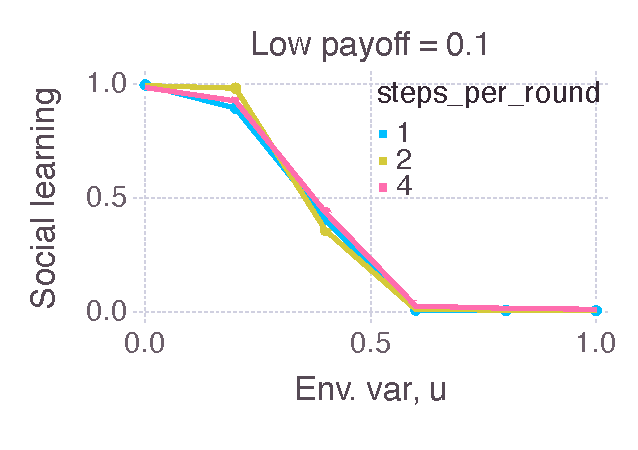
\includegraphics[width=\textwidth]{{Figures/SL_over_u_lowpayoff=0.1.pdf}}
  \caption{}
  \label{fig:}
  \end{subfigure}

  \begin{subfigure}[t]{0.5\textwidth}
    \centering
    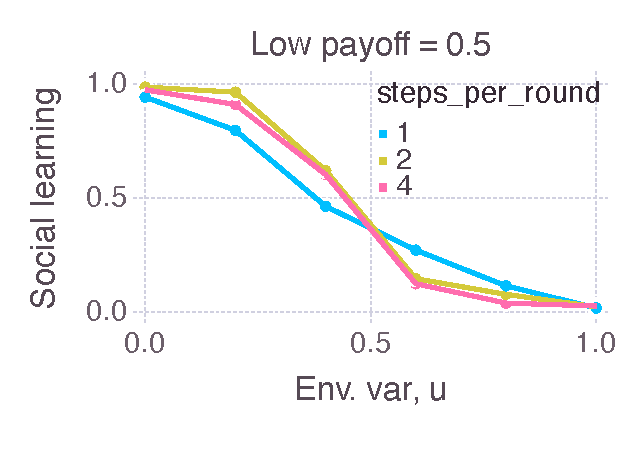
\includegraphics[width=\textwidth]{{Figures/SL_over_u_lowpayoff=0.5.pdf}}
  \caption{}
  \label{fig:}
  \end{subfigure}

  \begin{subfigure}[t]{0.5\textwidth}
    \centering
    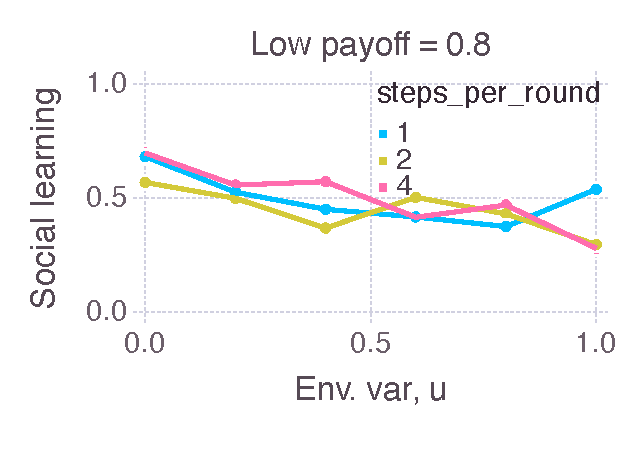
\includegraphics[width=\textwidth]{{Figures/SL_over_u_lowpayoff=0.8.pdf}}
  \caption{}
  \label{fig:}
  \end{subfigure}
  
  \caption{}
  \label{fig:}
\end{figure}


\section{Discussion}


\bibliographystyle{apacite}

\setlength{\bibleftmargin}{.125in}
\setlength{\bibindent}{-\bibleftmargin}

\bibliography{/Users/mt/workspace/Writing/library.bib}

\end{document}
